$\displaystyle \int_{0}^{1}\frac{arctg x}{x^2+1}\,dx$

\nopagebreak
\begin{align*}
\text{Sustitución: } u = \arctan x \implies du = \frac{dx}{x^2+1}. \\
\text{Límites: } x=0 \to u=0; \quad x=1 \to u=\pi/4. \\
I &= \int_{0}^{\pi/4} u \, du = \left[ \frac{u^2}{2} \right]_{0}^{\pi/4} \\
&= \frac{1}{2} \left(\frac{\pi}{4}\right)^2 - 0 = \frac{\pi^2}{32}
\end{align*}

\[
\boxed{\displaystyle \frac{\pi^2}{32}}
\]

\begin{center}
    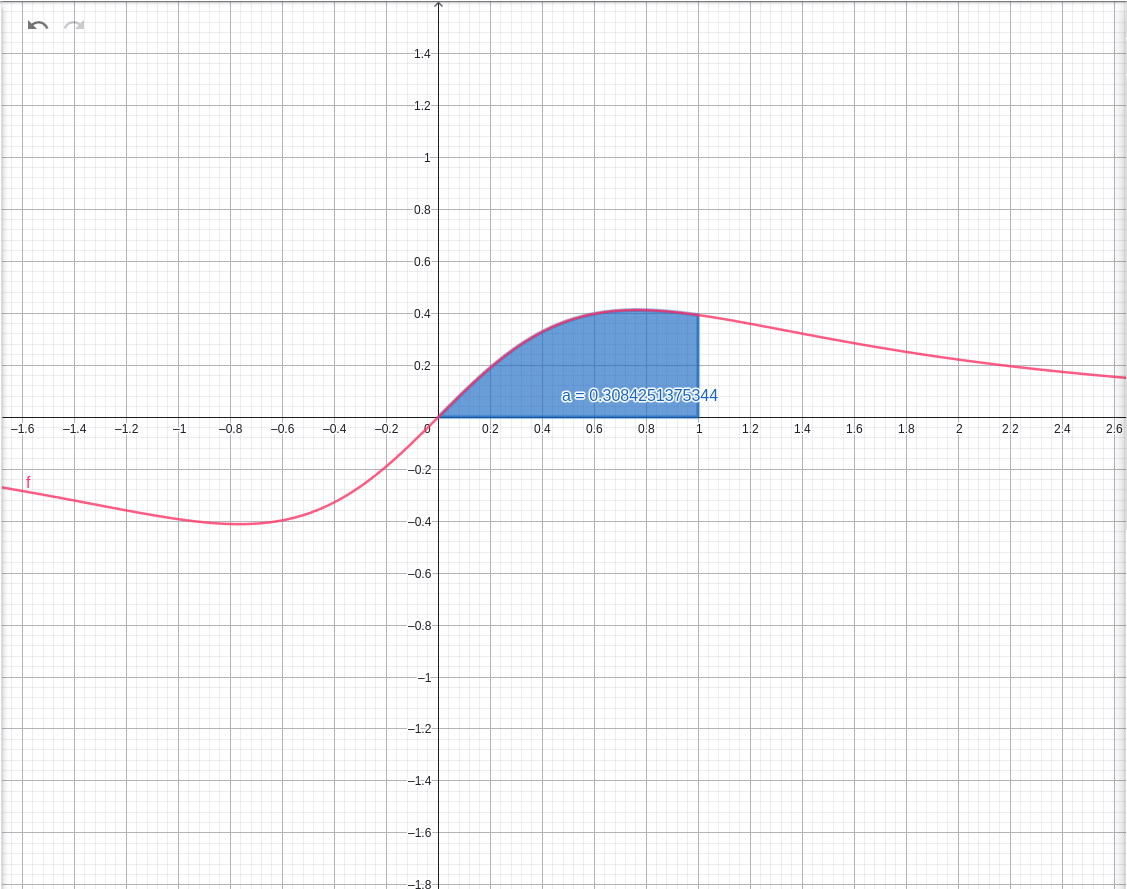
\includegraphics[width=0.5\textwidth]{Graficas/ejer14.png}
\end{center}
